\begin{center}
	{\Huge Coding/Core Module}
\end{center}

\setcounter{section}{0}
\section{Core Modules:}
\begin{center}
	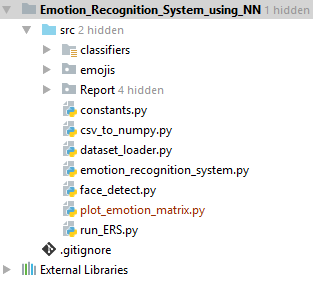
\includegraphics{Images/code_tree.png}
\end{center}

\textbf{face\_detect.py} - It is a script that runs on a input video stream may be on a video file or camera input , while using classifiers it detects the faces present in the video frame . The function in this file returns a NumPy array of detected faces per frame . These detected faces are then extracted out for further use.

\textbf{csv\_to\_numpy.py} - Since the data set provided to us is in CSV format , we need to convert that csv into numpy so that we can use it in our python module
The Dataset that we are using is radboud face dataset . This data set is the set of 64 Models having a set of 28,000 + pictures of people displaying 7 emotional expressions (angry, disgusted, fearful, happy, sad, surprised and neutral).

The dataset we are using consists of 2 types of data usages  - Training data and Test data. This script generates two models traing and test models . First one is used to train the machine and test data is used to verify the learning the machine.